\section{Caracterización y tests}

\begin{frame}
\begin{center}
\Huge CARACTERIZACIÓN Y PRUEBAS
\end{center}
\end{frame}

\begin{frame}{Listado de pruebas}
  \begin{itemize}
    \item<1-> Ensayos de verificación
    \begin{itemize}
      \Fontitit
      \item<2-> \color<10->[rgb]{0,0.6,0}Transformación de señales patrón
    \end{itemize}
    \item<3-> Ensayos de caracterización
    \begin{itemize}
      \Fontitit
      \item<4-> Medición del error
      \item<5-> Medición de la THD
      \item<6-> Efecto del escalamiento
      \item<7-> Medición de los recursos necesarios 
    \end{itemize}
    \item<8-> Ensayos de validación
    \begin{itemize}
      \Fontitit
      \item<9-> Implementación en FPGA
    \end{itemize}
  \end{itemize}
\end{frame}

\subsection{Señales Patrón}

\begin{frame}{Señales patrón}
  \uncover<1->{
  \begin{itemize}
    \item<1-> Se realizaron pruebas utilizando como entrada deltas en diferentes compoenentes y se
    analizó su salida
    \begin{itemize}
      \item<2-> Una delta en posición `0'
      \item<3-> Una delta en posición `6'
    \end{itemize}
  \end{itemize}
  }
  \uncover<2->{
    \alt<2>{
      \begin{center}
        \advance\leftskip-0.2cm
        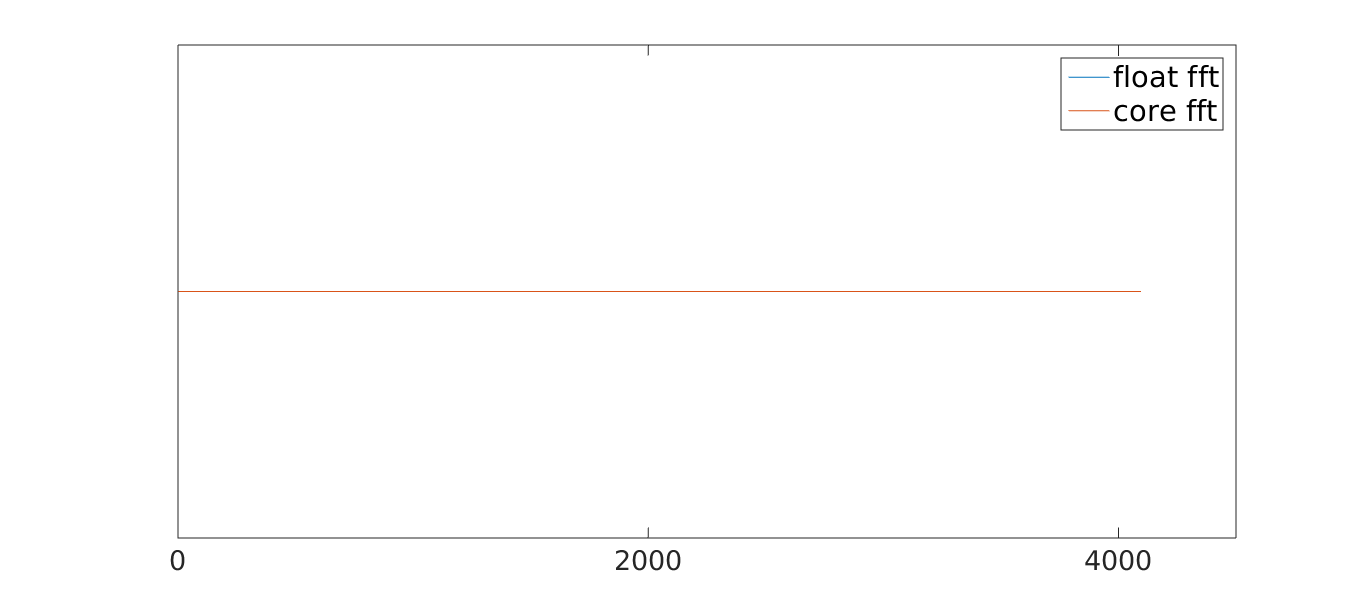
\includegraphics[scale=0.3]{./figures/r2_delta0_16_4096_mul.png}
      \end{center}
    }{
      \begin{center}
        \advance\leftskip-0.2cm
        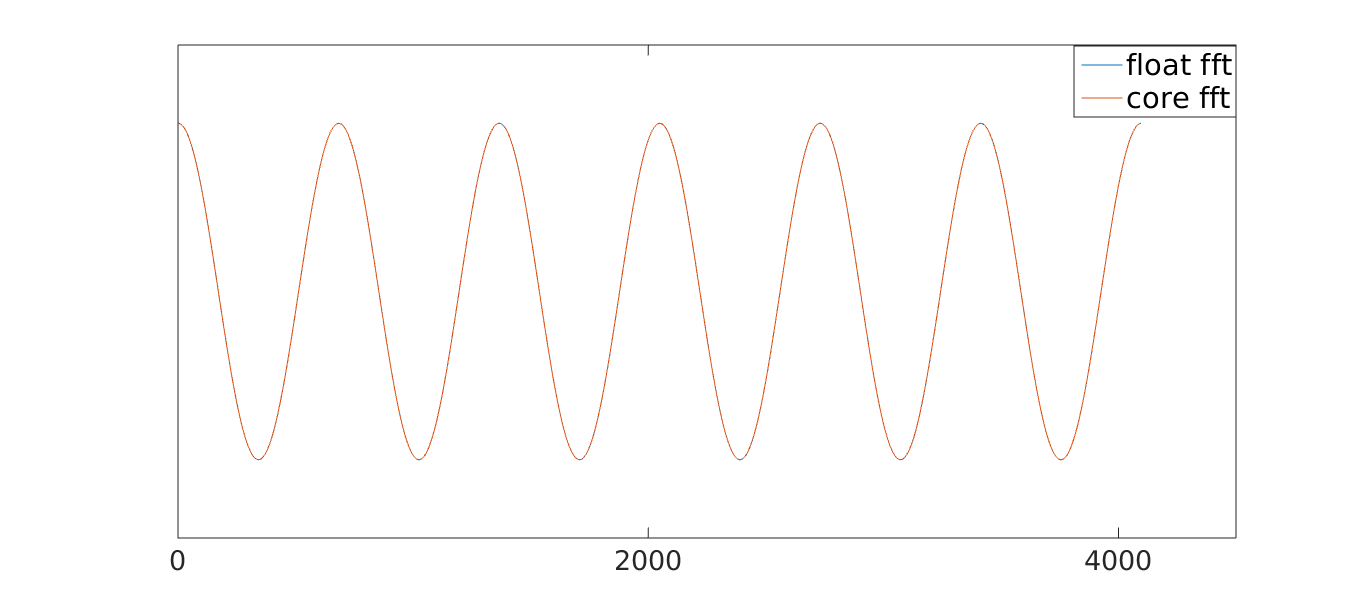
\includegraphics[scale=0.3]{./figures/r2_delta7_16_4096_mul.png}
      \end{center}
    }
  }
\end{frame}

\subsection{Medición del error}

\begin{frame}{}
  \begin{itemize}
    \item<1-> Ensayos de verificación
    \begin{itemize}
      \Fontitit
      \item<1-> Transformación de señales patrón
    \end{itemize}
    \item<1-> Ensayos de caracterización
    \begin{itemize}
      \Fontitit
      \item<1-> \color<1->[rgb]{0,0.6,0}Medición del error
      \item<1-> Medición de la THD
      \item<1-> Efecto del escalamiento
      \item<1-> Medición de los recursos necesarios 
    \end{itemize}
    \item<1-> Ensayos de validación
    \begin{itemize}
      \Fontitit
      \item<1-> Implementación en FPGA
    \end{itemize}
  \end{itemize}
\end{frame}

\begin{frame}{}%{Métricas de error}
%   \only<1-8>{
%   \begin{itemize}
%     \item<1-> Las métricas utilizadas para estimar el error fueron
%     \begin{itemize}
%       \item<2-> $E_\infty = MAX\left(\frac{ X_o[n] - X_{dut}[n]}{X_o[n]}\right)$
%       \item<3-> $E_2 = \left\Vert\frac{X_o[n] - X_{dut}[n]}{X_o[n]}\right\Vert_2$
%     \end{itemize}
%     \item<4-> Dado que el sistema es no lineal se realizaron 1024 simulaciones
%     \begin{itemize}
%       \item<5-> Se creó una entrada aleatoria para cada simulación
%       \item<6-> Se calculó el error en cada simulación y luego se promedió
%       \item<7-> Se realizó para cada arquitectura
%       \item<8-> Se utilizó el cálculo de FFT de la señal de entrada en Matlab como referencia para
%       el cálculo de error
%     \end{itemize}
%     \item<9-> Se contrastó con el error de una arquitectura de cómputo de FFT de terceros: KISS
%       FFT en C++
%   \end{itemize}
%   }
  
%  \only<9>{
    \begin{columns}[T]
      \begin{column}{.44\textwidth}
        \begin{center}
          \advance\leftskip-0.2cm
          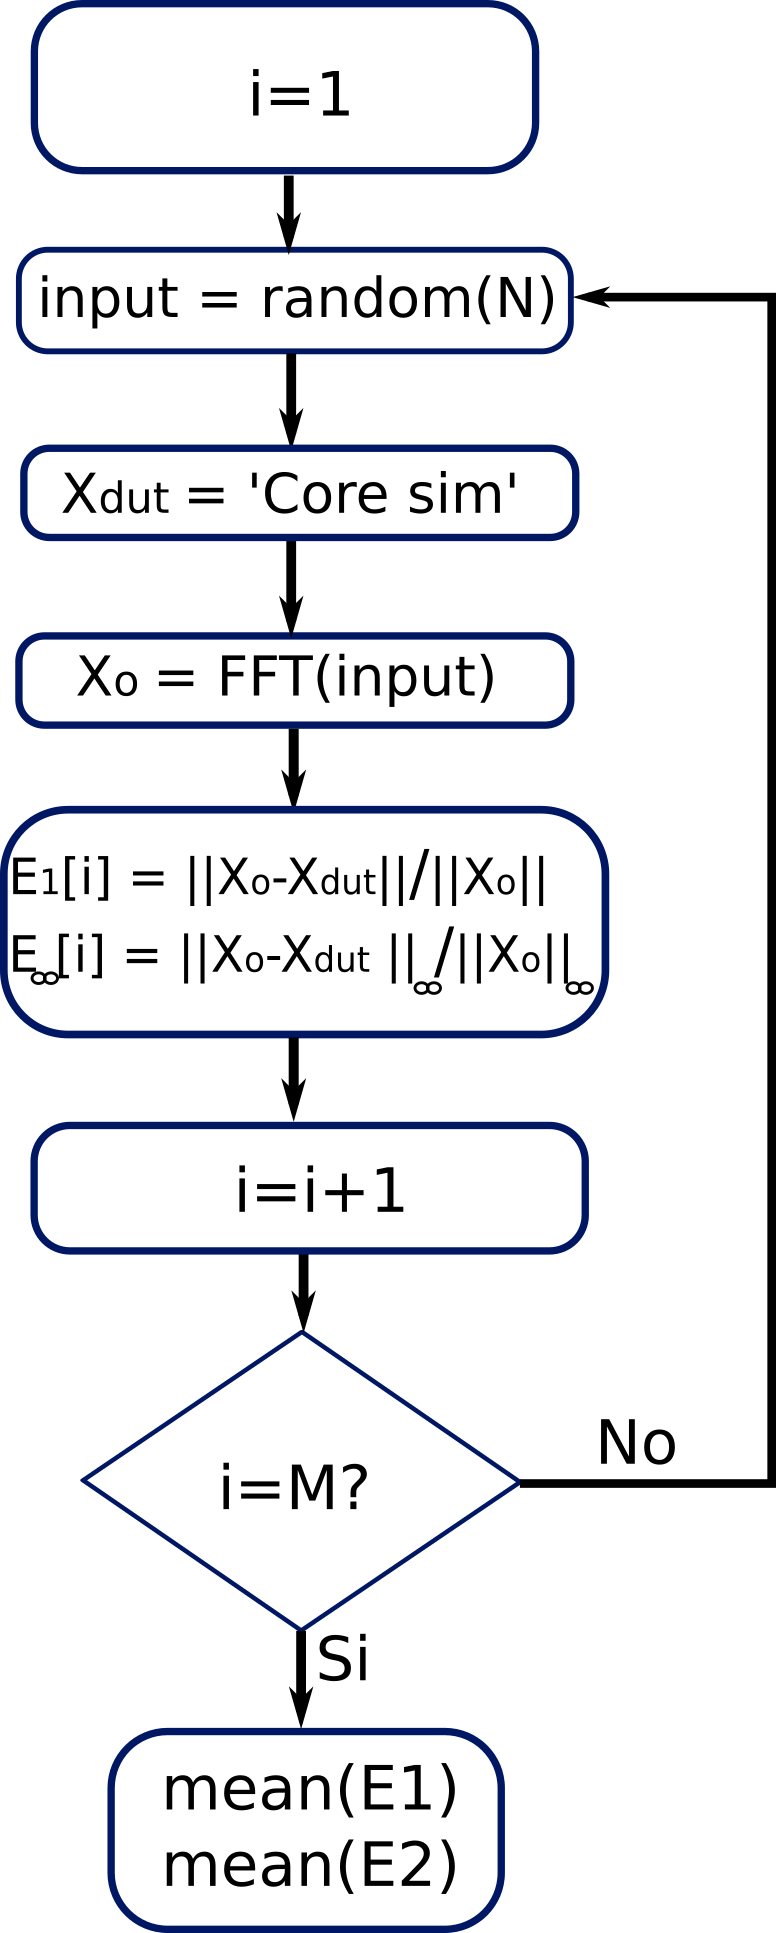
\includegraphics[scale=0.3]{./figures/error_sim.png}
        \end{center}
      \end{column}
      
      \begin{column}{.56\textwidth}
        \begin{center}
          \advance\leftskip-0.2cm
          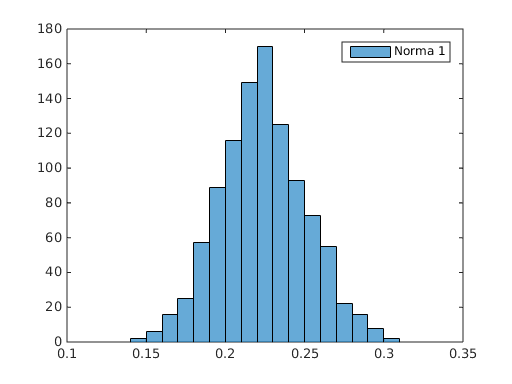
\includegraphics[scale=0.3]{./figures/norm1_1024_12.png}
        \end{center}
        
        \begin{center}
          \advance\leftskip-0.2cm
          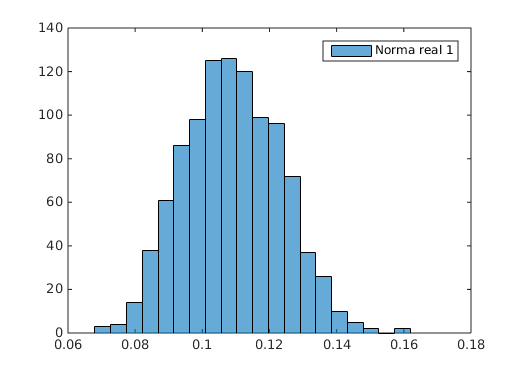
\includegraphics[scale=0.3]{./figures/norm1_r2_16_4096_mul.png}
          %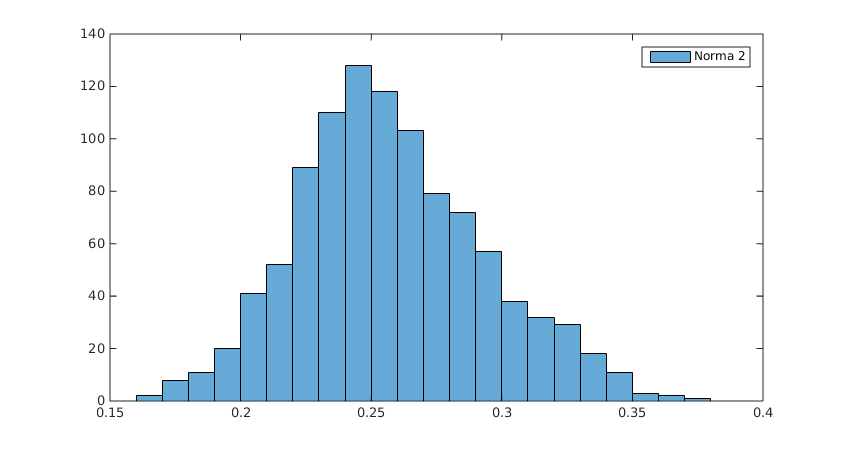
\includegraphics[scale=0.2]{./figures/norm2_1024_12.png}
        \end{center}
        
%         \begin{center}
%           \advance\leftskip-0.2cm
%           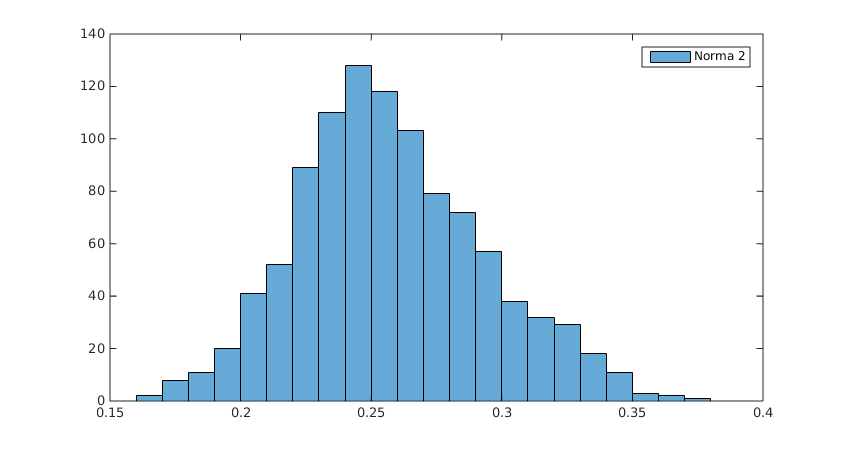
\includegraphics[scale=0.3]{./figures/norm2_1024_12.png}
%         \end{center}
      \end{column}
    \end{columns}
%    }
\end{frame}

\begin{frame}{Resultados de la medición de error}

  \begin{columns}[T]
    \begin{column}{.2\textwidth}

    \end{column}
    \begin{column}{.8\textwidth}
	\begin{tabular}{l c c c c}
		& \textbf{1024, 12} & \textbf{1024, 16} & \textbf{4096, 12} & \textbf{4096, 16}\\ \hline 
		\textbf{R-2, cordic} & $0.092$ & $0.006$ & $0.099$ & $0.008 $\\
		\textbf{R-2, Mult.} & $0.232$ & $0.003$ & $0.340$ & $0.108$\\
		\textbf{R-4, cordic} & $0.077$ & $0.003$ & $0.074$ & $0.007$\\
		\textbf{R-4, Mult.} & $0.224$ & $0.002$ & $0.334$ & $0.105$\\
		\textbf{Kiss FFT} & $ $ & $0.017$ & $ $ & $0.035$\\
		\textbf{Xilinx FFT v7.1} & $0.0007$ & $0.0001$ & $0.0008$ & $0.0004$\\ \hline
	\end{tabular}\\
	\end{column}
	
	\begin{column}{.2\textwidth}
	
	\end{column}

  \end{columns}
	
% 	Resultados para $E_2$
% 	\begin{tabular}{l c c c c }
% 		 & \textbf{1024, 12} & \textbf{1024, 16} & \textbf{4096, 12} & \textbf{4096, 16}\\ \hline 
% 		\textbf{R-2, cordic} & $0.095$ & $0.007$ & $0.116$ & $0.053$\\
% 		\textbf{R-2, Mult.} & $0.257$ & $0.004$ & $0.356$ & $0.131$\\
% 		\textbf{R-4, cordic} & $0.084$ & $0.002$ & $0.094$ & $0.027$\\
% 		\textbf{R-4, Mult.} & $0.258$ & $0.003$ & $0.358$ & $0.126$\\ 
% 		\textbf{Kiss FFT} & $ $ & $0.017$ & $ $ & $0.035$\\\hline
% 	\end{tabular}

\end{frame}

\subsection{Medición de la THD}

\begin{frame}{}
  \begin{itemize}
    \item<1-> Ensayos de verificación
    \begin{itemize}
      \Fontitit
      \item<1-> Transformación de señales patrón
    \end{itemize}
    \item<1-> Ensayos de caracterización
    \begin{itemize}
      \Fontitit
      \item<1-> Medición del error
      \item<1-> \color<1->[rgb]{0,0.6,0}Medición de la THD
      \item<1-> Efecto del escalamiento
      \item<1-> Medición de los recursos necesarios 
    \end{itemize}
    \item<1-> Ensayos de validación
    \begin{itemize}
      \Fontitit
      \item<1-> Implementación en FPGA
    \end{itemize}
  \end{itemize}
\end{frame}

\begin{frame}{Medición de la THD}
%   \only<1-5>{
%   \begin{itemize}
%     \item<1-> Las arquitecturas se comportan como sistemas no lineales
%     \item<2-> Para medir completamente la THD no alcanza con medir para algunas frecuencias
%     \item<3-> Se midió la THD para entradas delta en cada una de las componentes para cada
%     arquitectura
%     \item<4-> Se tomó la salida de cada simulación y se calculó la THD mediante Matlab.
%     \item<5-> Se contrastó con la THD de la arquitectura Kiss FFT en C++.
%   \end{itemize}
%   }
  
%  \only<6>{
    \begin{center}
      \advance\leftskip-0.2cm
      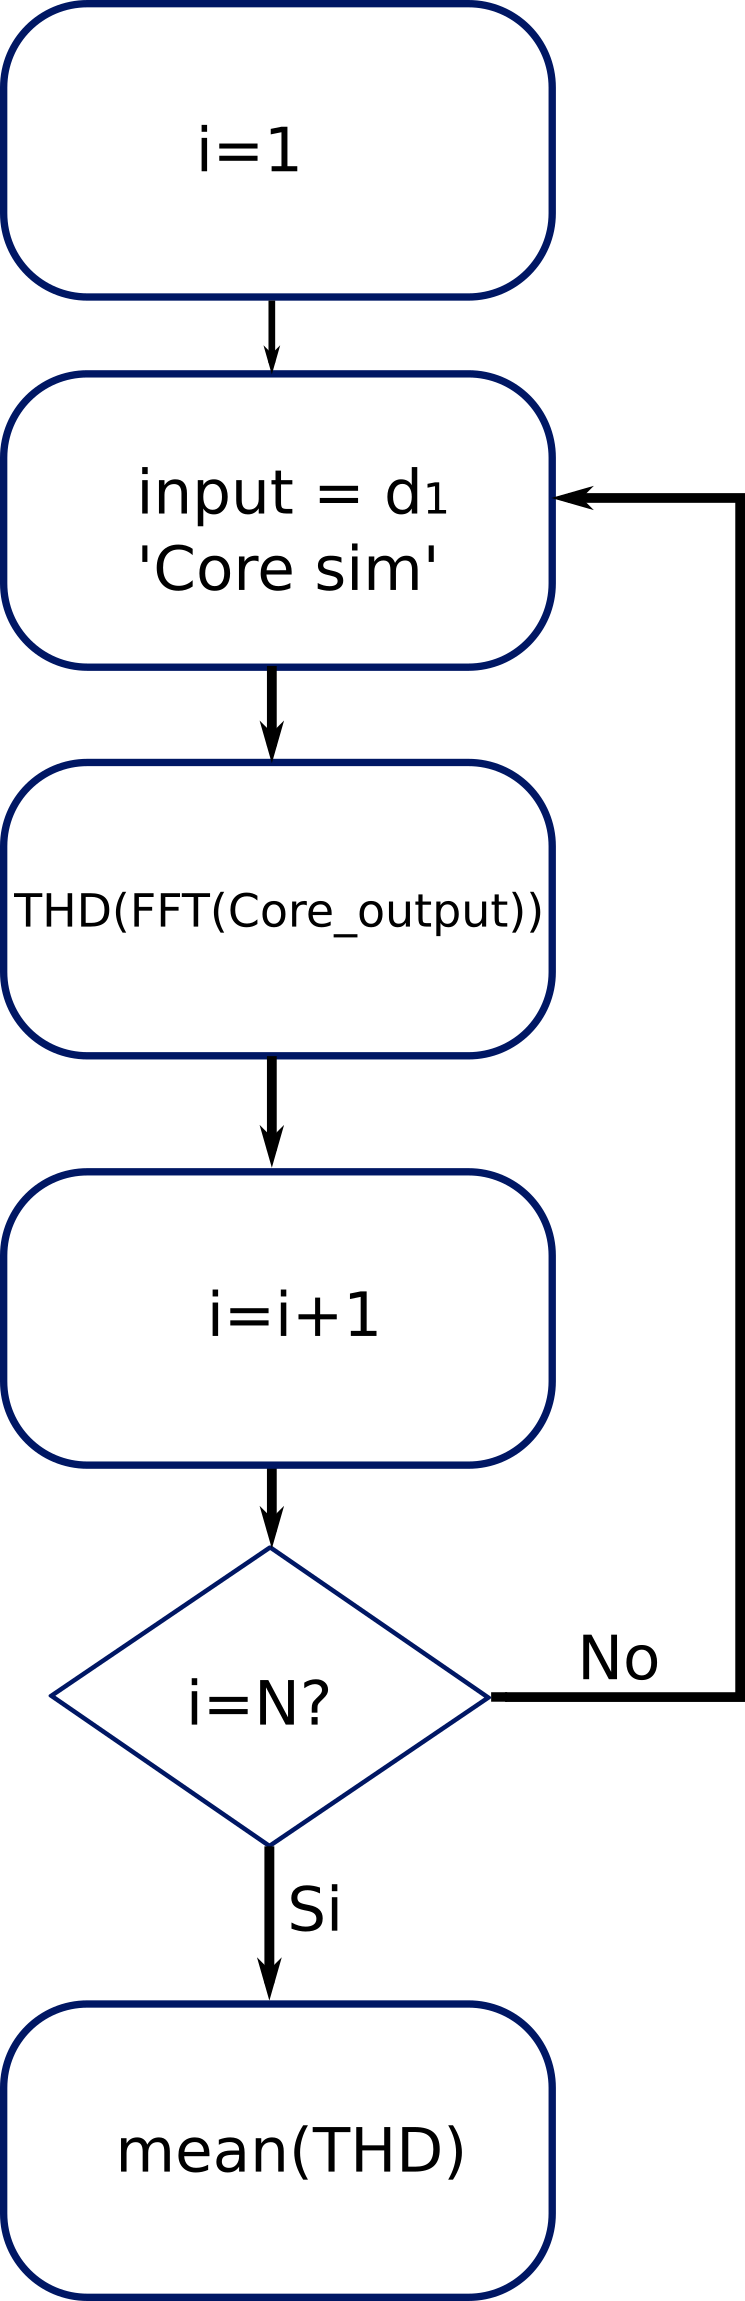
\includegraphics[scale=0.27]{./figures/thd_sim.png}
    \end{center}
%  }  
\end{frame}

\begin{frame}{THD - Resultados}
  \begin{columns}[T]
    \begin{column}{.5\textwidth}
      %\only<1-1>{
        \begin{center}
	      %\advance\leftskip-0.2cm
	      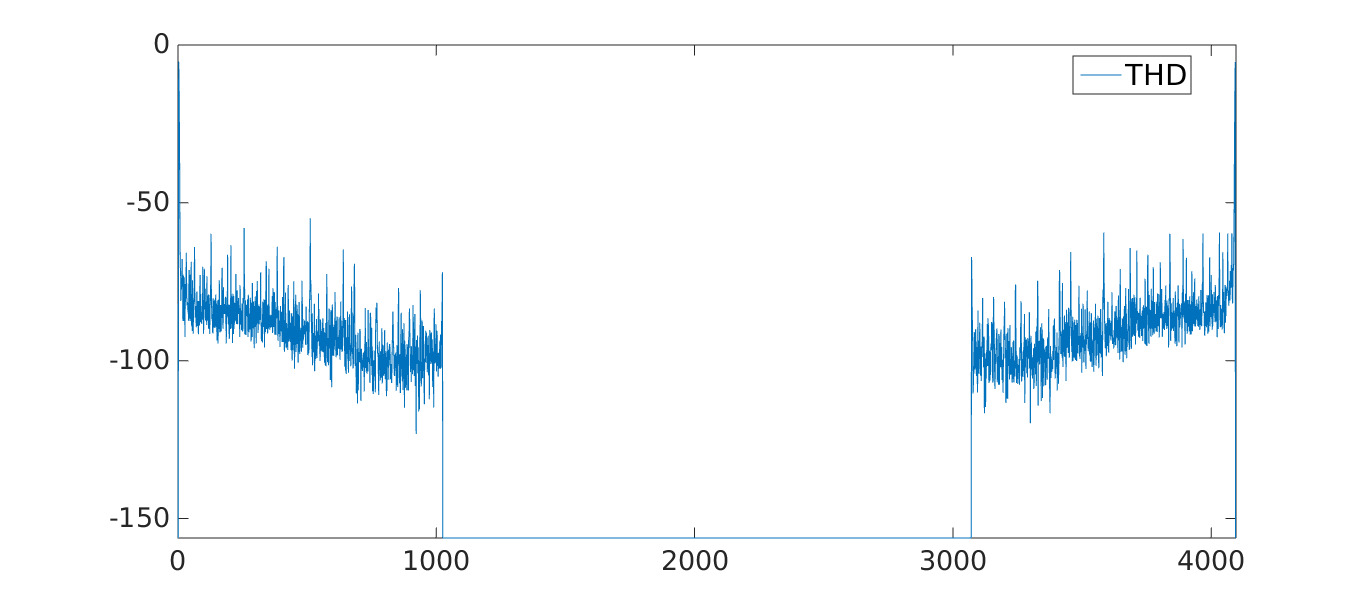
\includegraphics[scale=0.17]{./figures/thd_r2_4096_16_cor.png}\\
          Radix-2, Cordic, 16 bits
        \end{center}
       % }
	    
	    
	    \begin{center}
	      %\advance\leftskip-0.2cm
	      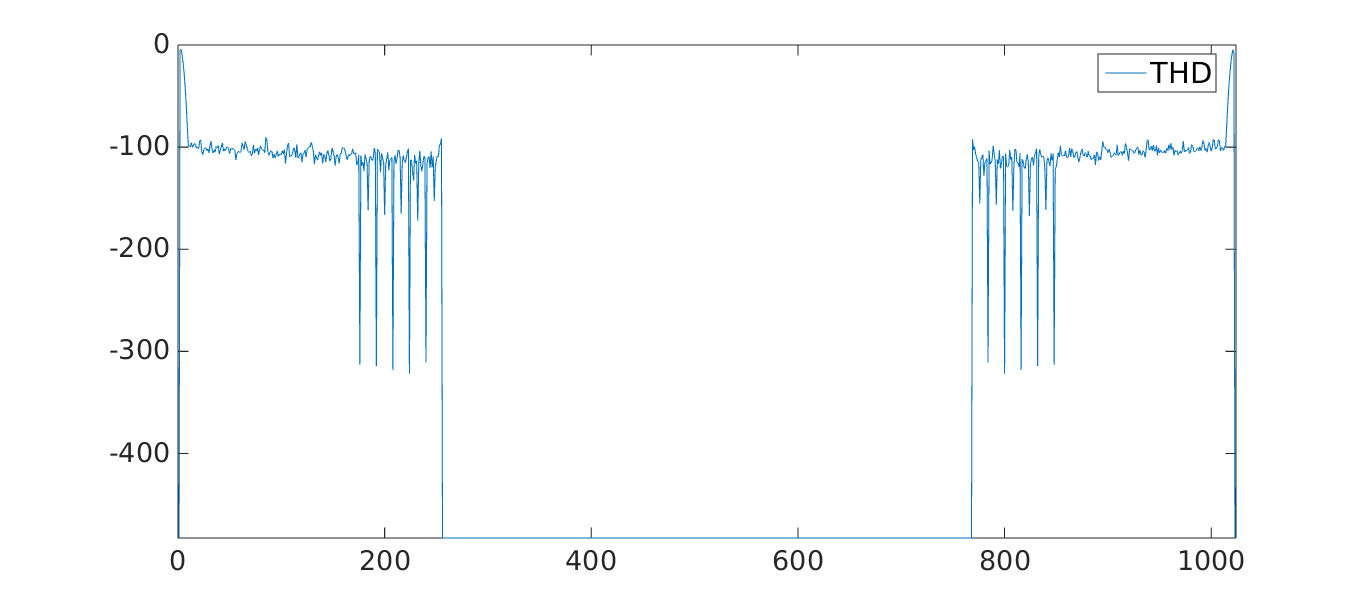
\includegraphics[scale=0.17]{./figures/thd_r4_1024_16_mul.png}\\
	      Radix-4, Mult., 16 bits
	    \end{center}
	    
	  %\only<2-2>{  
% 	    \begin{center}
% 	      %\advance\leftskip-0.2cm
% 	      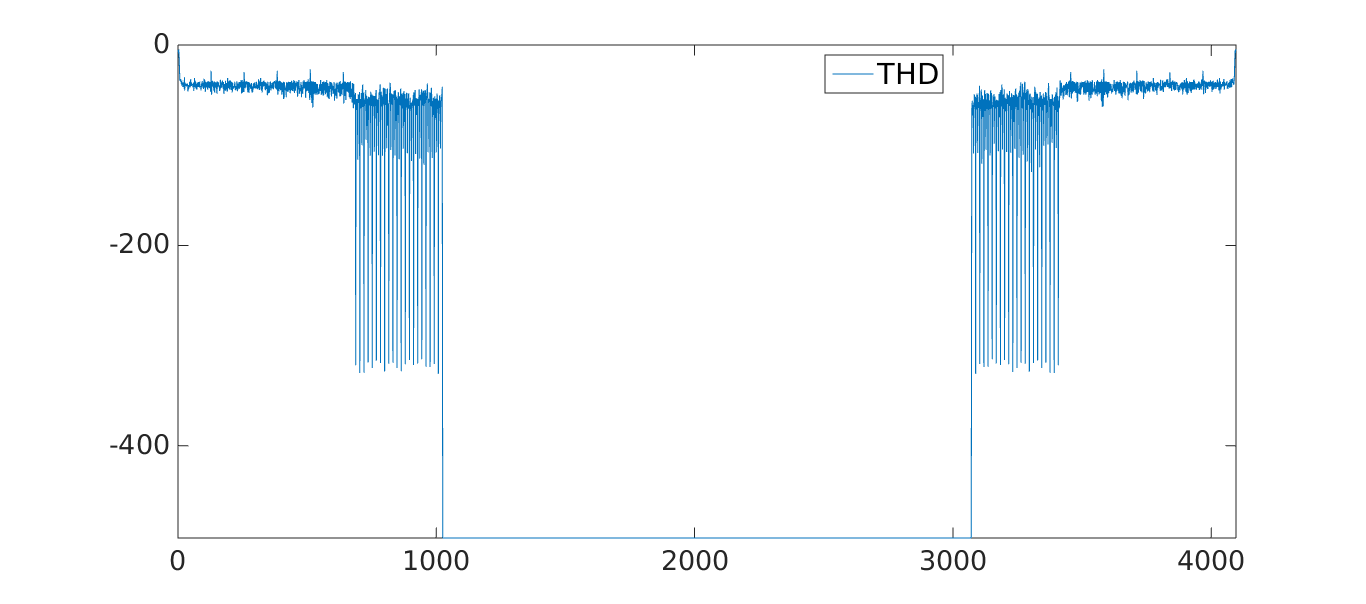
\includegraphics[scale=0.15]{./figures/thd_kiss_4096_16.png}\\
% 	      Kiss FFT. C++. 16 bits
% 	    \end{center}
	  %}
	    
    \end{column}
    
    \begin{column}{.5\textwidth}
%       \only<1-1>{
%         \begin{center}
% 	      %\advance\leftskip-0.2cm
% 	      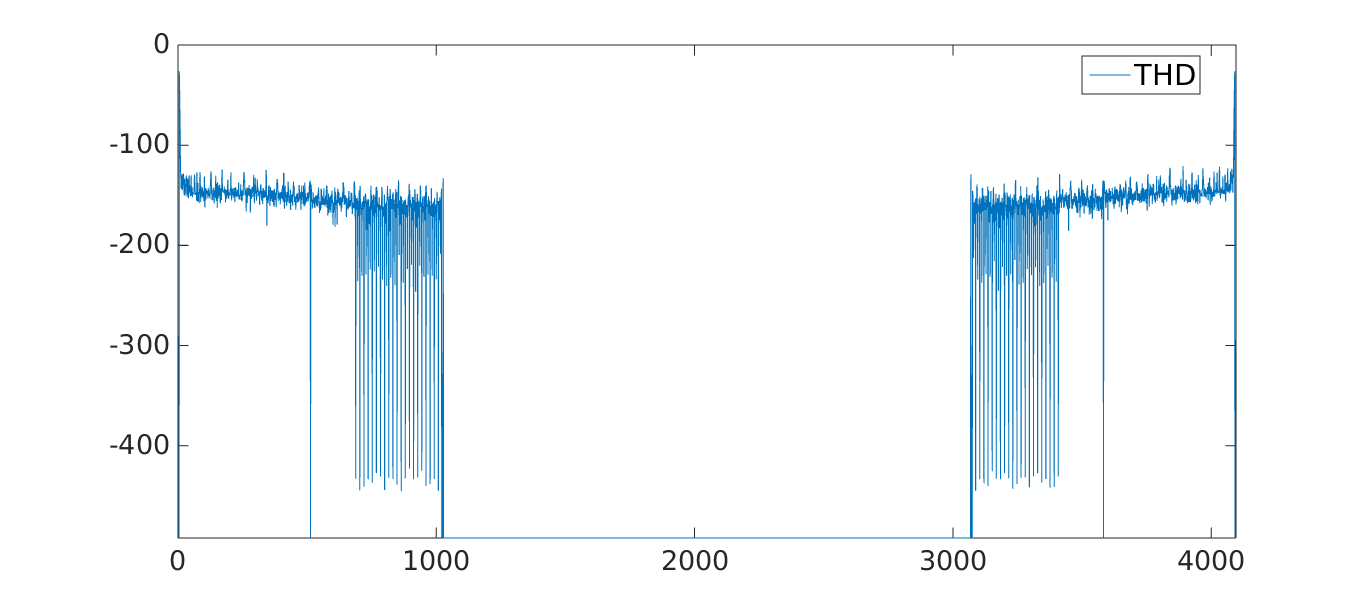
\includegraphics[scale=0.15]{./figures/thd_r2_4096_16_mul.png}\\
% 	      Radix-2, Mult., 16 bits
% 	    \end{center}
% 	    }
	    
	    
	    \begin{center}
	      %\advance\leftskip-0.2cm
% 	      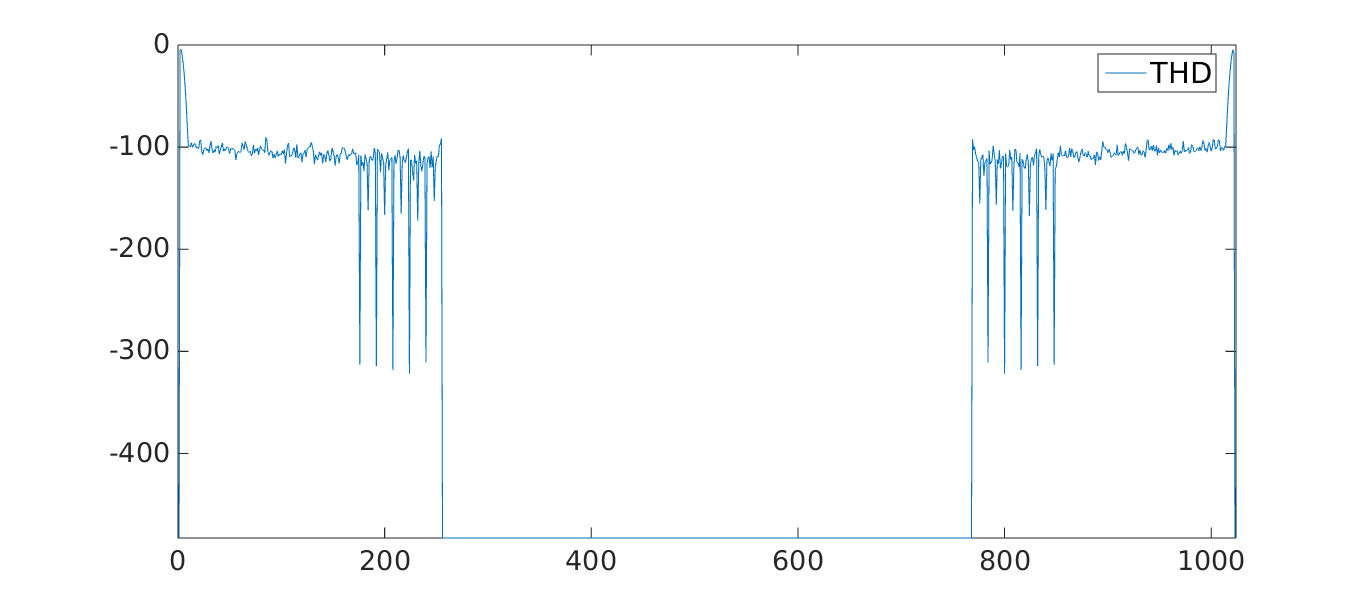
\includegraphics[scale=0.15]{./figures/thd_r4_1024_16_mul.png}\\
% 	      Radix-4, Mult., 16 bits
	       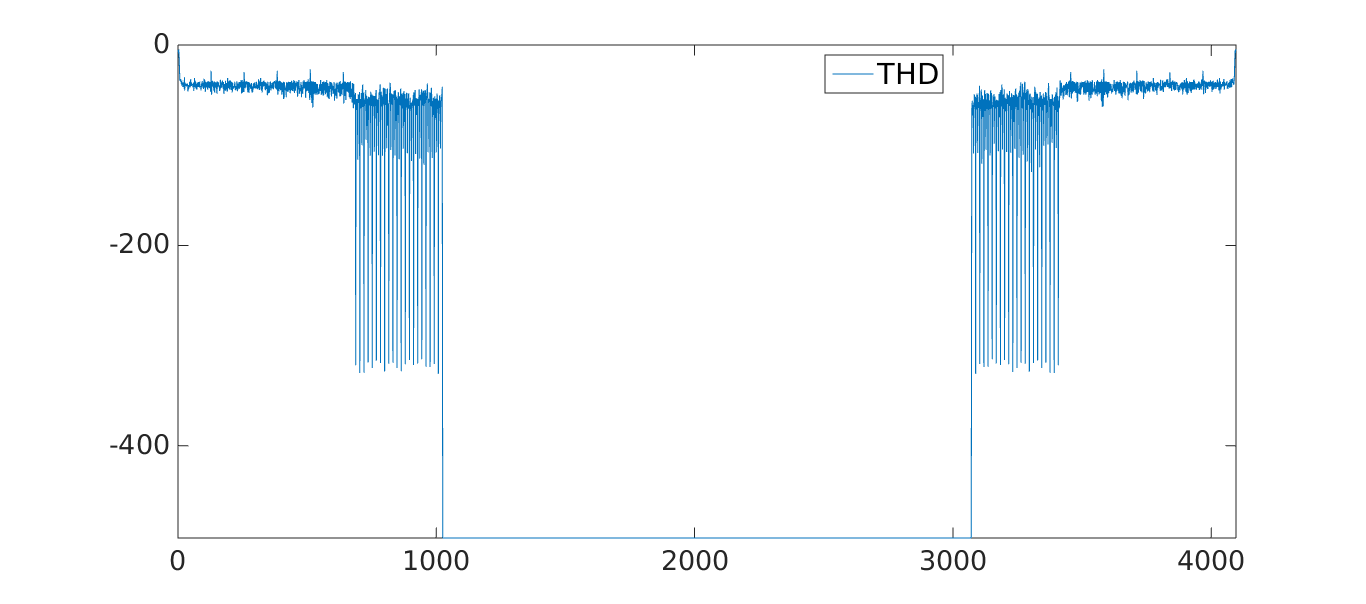
\includegraphics[scale=0.17]{./figures/thd_kiss_4096_16.png}\\
	      Kiss FFT. C++. 16 bits
	    \end{center}
	    
%	  \only<2-2>{  
	    \begin{center}
	      %\advance\leftskip-0.2cm
	      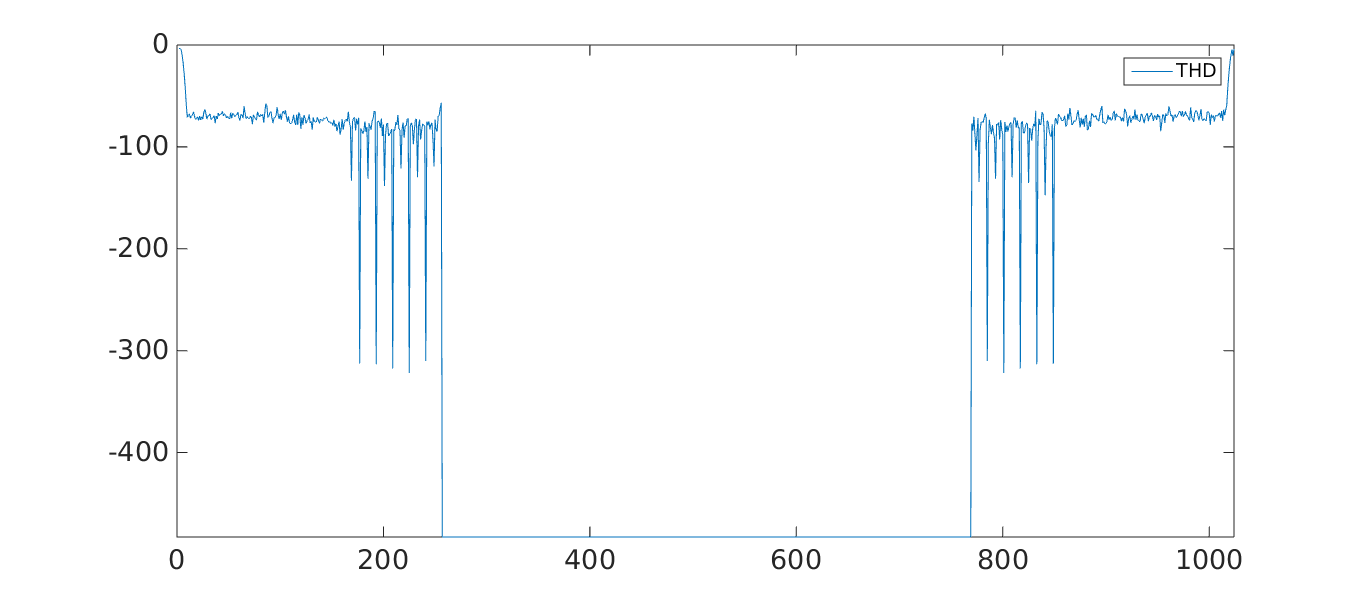
\includegraphics[scale=0.17]{./figures/thd_xilinx_r4_16_1024.png}\\
	      Xilinx LogiCORE FFT 7.1
	      %Matlab. Punto flotante 64 bits
	    \end{center}
%	  }
	    
    \end{column}
  \end{columns}
\end{frame}

% \begin{frame}{Análisis de la intermodulación}
% %   \begin{itemize}
% %     \item<1-> Se midió la THD para un tono determinado
% %     \item<2-> Se midió la THD para una señal que contiene el mismo tono y el tono inmediato
% %     anterior, y se comparó con la THD anterior
% %   \end{itemize}
% %   \uncover<3-4>{
% %   \begin{columns}[T]
% %     \begin{column}{.5\textwidth}
% % \begin{itemize}
% %   \item<1-> Señal que produce overflow 
%       \begin{center}
%         \advance\leftskip-0.2cm
% 	    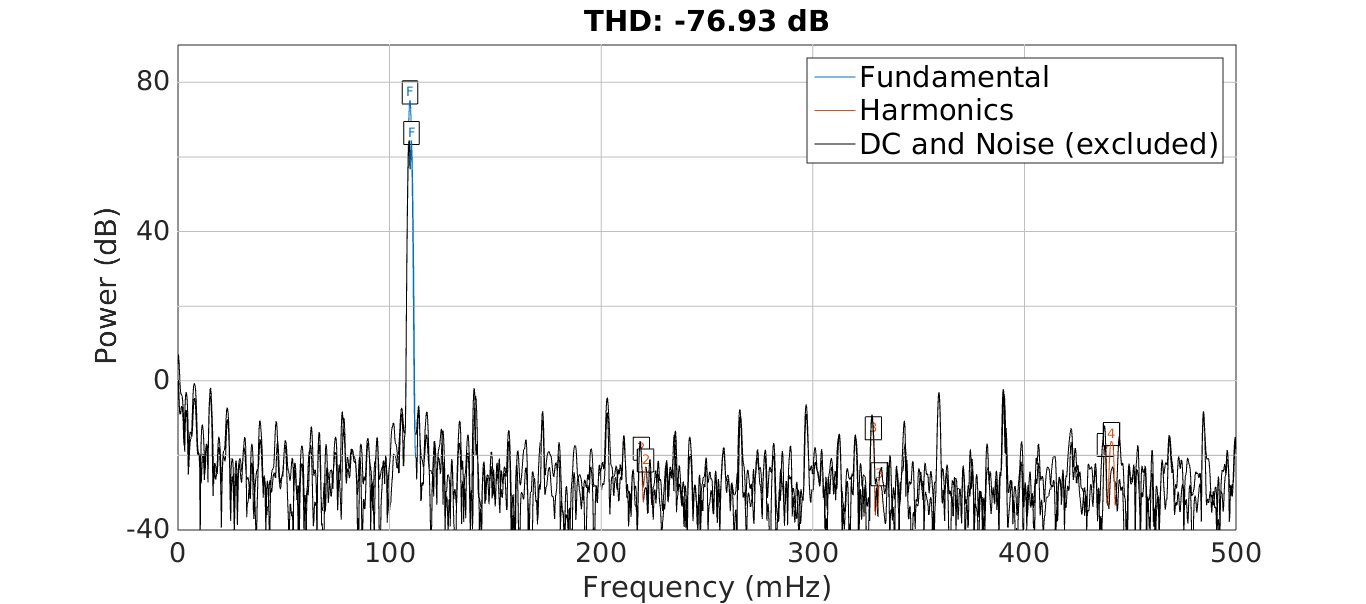
\includegraphics[scale=0.22]{./figures/thd_r2_4096_16_cor_450_451.png}\\
% 	    Rotador Cordic.
% 	  \end{center}
% % 	\end{column}
% 	
% % 	\begin{column}{.5\textwidth}
% %   \item<2-> Señal con produce overflow
% 	  \begin{center}
% 	    \advance\leftskip-0.2cm
% 	    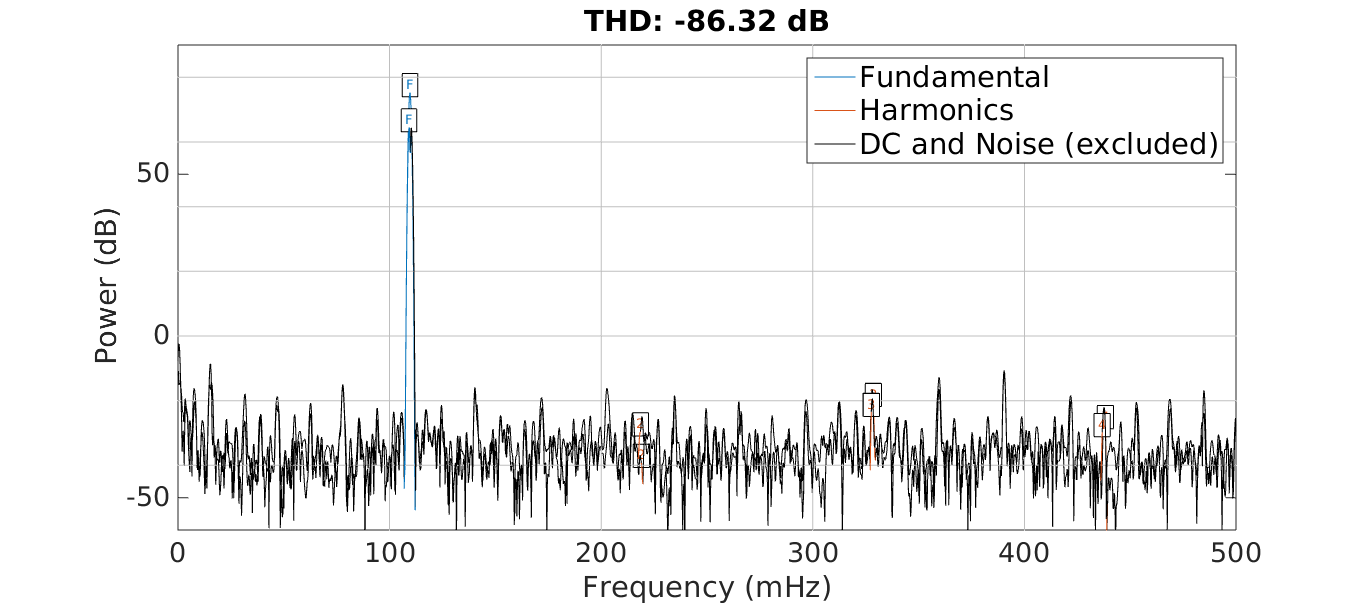
\includegraphics[scale=0.22]{./figures/thd_r2_4096_16_mul_450_451.png}\\
% 	    Multiplicador complejo.
% 	  \end{center}
% % 	\end{column}
% %   \end{columns}
% %   }
% %   \begin{itemize}
% %     \item<4-4> Se observa que no hay efectos de intermodulación 
% %   \end{itemize}
% \end{frame}

\subsection{Efecto del escalamiento}

\begin{frame}{}
  \begin{itemize}
    \item<1-> Ensayos de verificación
    \begin{itemize}
      \Fontitit
      \item<1-> Transformación de señales patrón
    \end{itemize}
    \item<1-> Ensayos de caracterización
    \begin{itemize}
      \Fontitit
      \item<1-> Medición del error
      \item<1-> Medición de la THD
      \item<1-> \color<1->[rgb]{0,0.6,0}Efecto del escalamiento
      \item<1-> Medición de los recursos necesarios 
    \end{itemize}
    \item<1-> Ensayos de validación
    \begin{itemize}
      \Fontitit
      \item<1-> Implementación en FPGA
    \end{itemize}
  \end{itemize}
\end{frame}

\begin{frame}{Efecto sobre la señal de salida}
  \begin{itemize}
    \item<1-> Provoca un escalamiento por $1/2$ por cada etapa donde se realiza escalamiento
    \item<2-> Provoca una pérdida de información
  \end{itemize}
  
  \uncover<3-3>{
    \begin{center}
      \advance\leftskip-0.2cm
      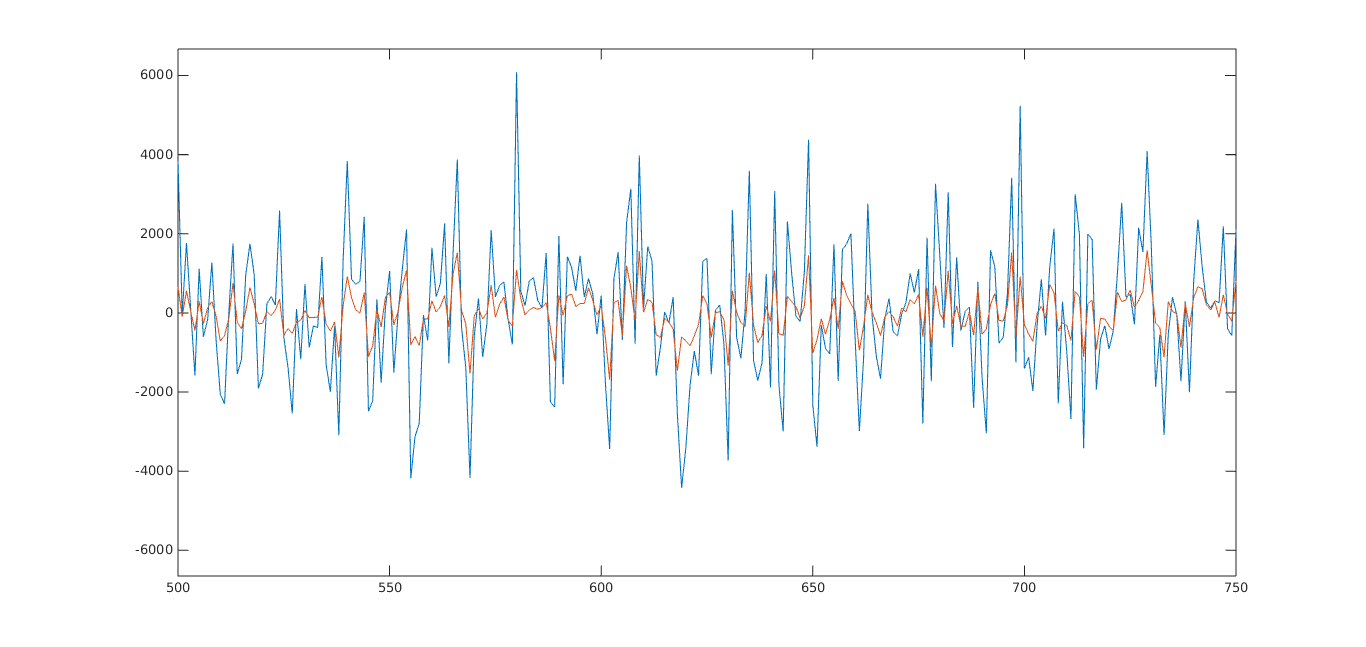
\includegraphics[scale=0.32]{./figures/rand_r2_16_4096_mul_trunc_2.png}\\
    \end{center}
    }
\end{frame}

\begin{frame}{Utilidad en caso de overflow}
  \begin{itemize}
%     \item<1-> Se utilizaron dos señales compuestas por una delta en una componente
%     \item<2-> Una dentro del rango de funcionamiento seguro y una que provoca overflow
%     \item<3-> Se simuló con escalamiento en cada etapa y se midió la THD en cada caso
%   \end{itemize}
%   
%   \uncover<4-4>{
%   \begin{columns}[T]
%     \begin{column}{.5\textwidth}
     \item<1-> Señal sin producir overflow
	  \begin{center}
		  \advance\leftskip-0.2cm
		  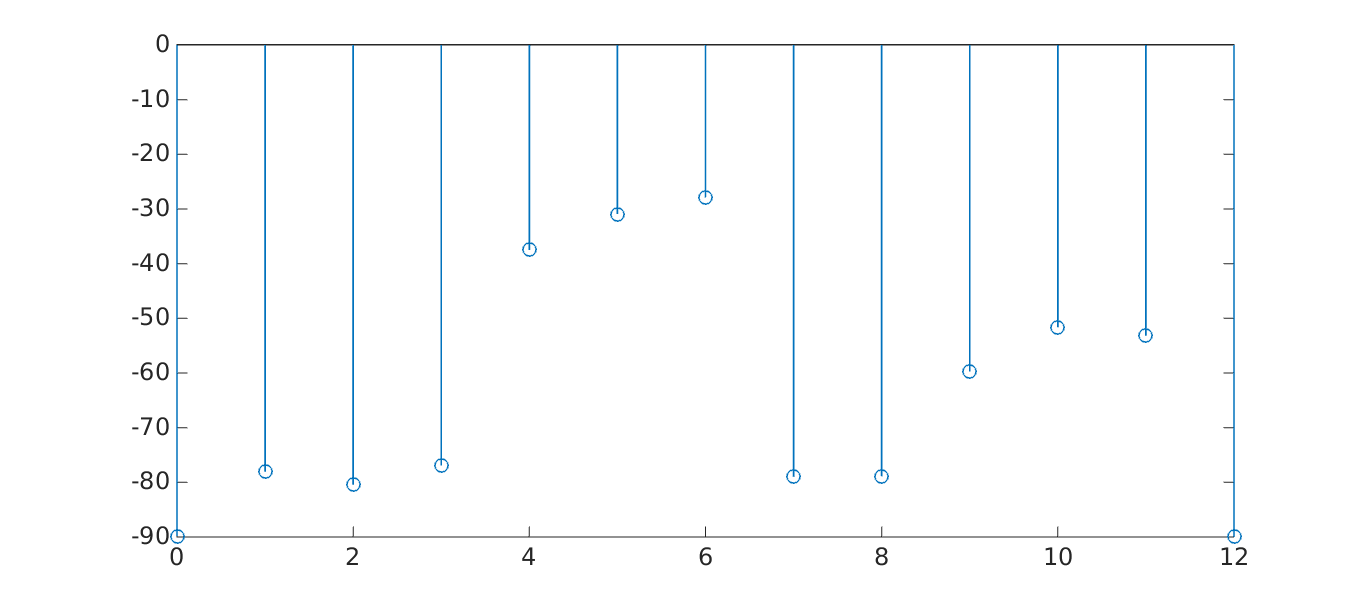
\includegraphics[scale=0.21]{./figures/r2_16_4096_mul_scale_thd_red.png}
		\end{center}
%     \end{column}
%     \begin{column}{.5\textwidth}
      \item<2-> Señal que provoca overflow
		\begin{center}
		  \advance\leftskip-0.2cm
		  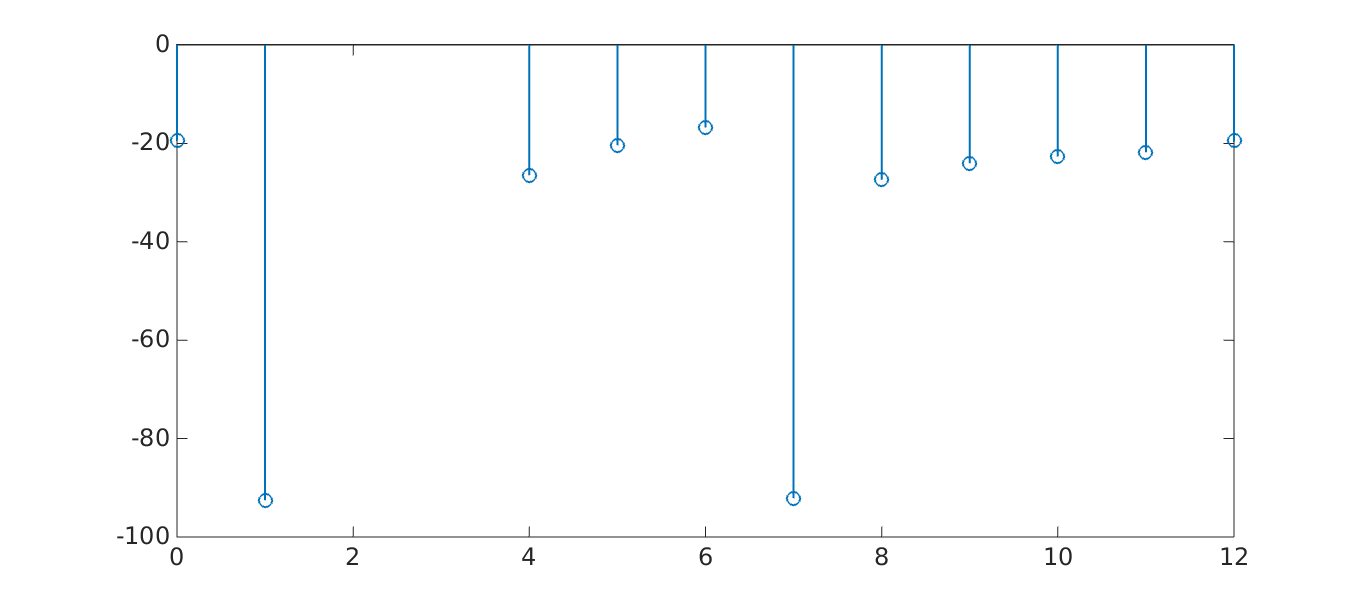
\includegraphics[scale=0.21]{./figures/r2_16_4096_mul_scale_thd_05_red.png}
		\end{center}
    \end{itemize}
% 	\end{column}
%   \end{columns}
%   }
\end{frame}

\subsection{Recursos de Implementación}

\begin{frame}{}
  \Fontit
  \begin{itemize}
    \item<1-> Ensayos de verificación
    \begin{itemize}
      \Fontitit
      \item<1-> Transformación de señales patrón
    \end{itemize}
    \item<1-> Ensayos de caracterización
    \begin{itemize}
      \Fontitit
      \item<1-> Medición del error
      \item<1-> Medición de la THD
      \item<1-> Efecto del escalamiento
      \item<1-> \color<1->[rgb]{0,0.6,0}Medición de los recursos necesarios 
    \end{itemize}
    \item<1-> Ensayos de validación
    \begin{itemize}
      \Fontitit
      \item<1-> Implementación en FPGA
    \end{itemize}
  \end{itemize}
\end{frame}

\begin{frame}{Recursos de implementación}
    \begin{columns}[T]
      \begin{column}{.53\textwidth}
      \begin{itemize}
        \item<1-> Uno de los requerimientos es la economía de recursos
        \item<2-> FPGA XC5VLX110, de la familia Virtex-5 de Xilinx.
        \item<3-> Se comparó con dos arquitecturas
        \begin{itemize}
          \item<4-> Radix-2 desenrrollada
          \item<5-> Xilinx LogiCORE FFT 7.1
        \end{itemize}
      \end{itemize}
      \end{column}
      \begin{column}{.47\textwidth}
        \centering
        \begin{center}
		  \advance\leftskip-0.2cm
		  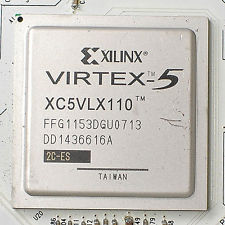
\includegraphics[scale=0.32]{./figures/virtex_chip.jpg}
		\end{center}
      \end{column}
    \end{columns}
%   \end{itemize}
\end{frame}

\begin{frame}{Resultados para 1024 puntos}
%  \uncover<3-3>{
%   \begin{columns}[T]
%     \begin{column}{.5\textwidth}

	  \begin{center}
		  %\advance\leftskip-0.2cm
		  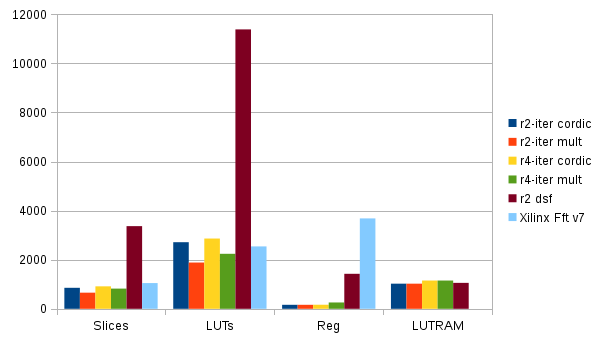
\includegraphics[scale=0.72]{./figures/sizecomp1024.png}\\
		  
		\end{center}
%     \end{column}
\end{frame}

\begin{frame}{Resultados para 4096 puntos}
%     \begin{column}{.5\textwidth}
		\begin{center}
		  %\advance\leftskip-0.2cm
		  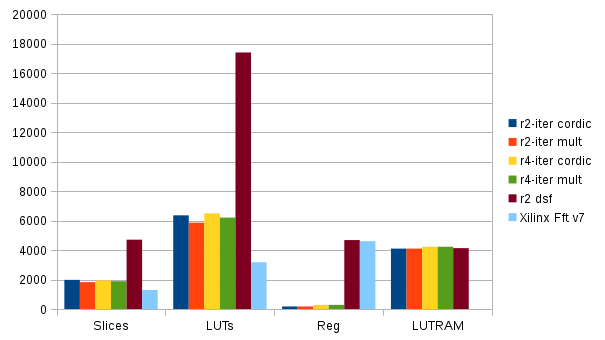
\includegraphics[scale=0.72]{./figures/sizecomp4096.png}\\
		\end{center}
% 	\end{column}
%   \end{columns}
%   }
\end{frame}

\subsection{Implementación en hardware}

\begin{frame}{}%{Listado de pruebas}
  \Fontit
  \begin{itemize}
    \item<1-> Ensayos de verificación
    \begin{itemize}
      \Fontitit
      \item<1-> Transformación de señales patrón
    \end{itemize}
    \item<1-> Ensayos de caracterización
    \begin{itemize}
      \Fontitit
      \item<1-> Medición del error
      \item<1-> Medición de la THD
      \item<1-> Efecto del escalamiento
      \item<1-> Medición de los recursos necesarios 
    \end{itemize}
    \item<1-> Ensayos de validación
    \begin{itemize}
      \Fontitit
      \item<1-> \color<1->[rgb]{0,0.6,0}Implementación en FPGA
    \end{itemize}
  \end{itemize}
\end{frame}

\begin{frame}{Validación en hardware}
  \only<1-2,4-5>{
    
      \begin{columns}[T]
        \begin{column}{.5\textwidth}
          \begin{itemize}
            \item<1-> Se un placa de desarrollo Avnet, con una FPGA XC5VLX110
            \item<2-> Se implementó adicionalmente una unidad de comuniación UART y una memoria
       auxiliar.
          \end{itemize}
        \end{column}
        \begin{column}{.5\textwidth}
          \centering
          \begin{center}
		    \advance\leftskip-0.2cm
		    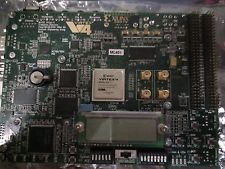
\includegraphics[scale=0.48]{./figures/virtex_board.jpg}
		  \end{center}
        \end{column}
      \end{columns}
      \begin{itemize}
        \item<4-> Se utilizaron como entrada las señales patrón ya utilizadas previamente, y señales
        aleatorias para las que se calculó el error.
        \item<5-> Los resultados de las corridas fueron similares al obtenido previamente en las
        simulaciones
      \end{itemize}
  }
  
  \only<3-3>{
    \begin{center}
	  \advance\leftskip-0.2cm
	  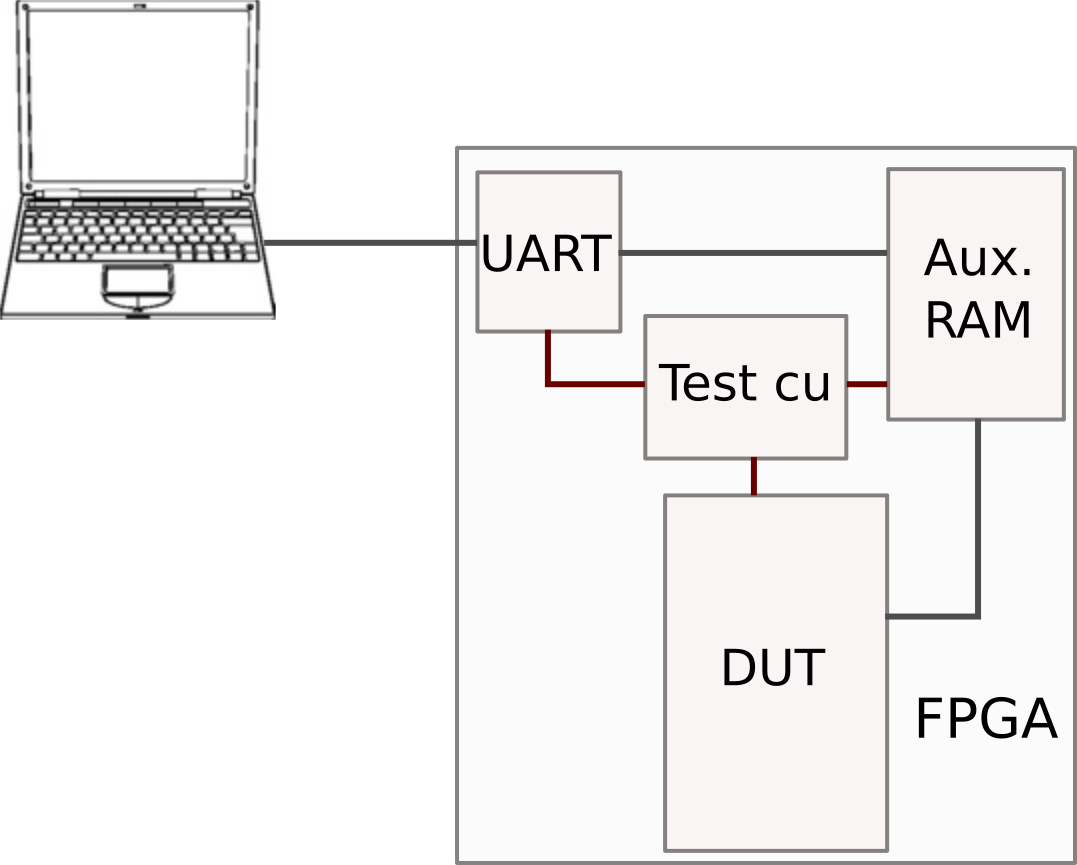
\includegraphics[scale=0.38]{./figures/hw_tb.png}\\
	\end{center}
  }
\end{frame}
